% ------------------------------------------------------------------------------
% TYPO3 Version 10.0 - What's New (Serbian Version)
%
% @author	Michael Schams <schams.net>
% @license	Creative Commons BY-NC-SA 3.0
% @link		http://typo3.org/download/release-notes/whats-new/
% @language	Serbian
% ------------------------------------------------------------------------------

\section{Administratorski interfejs}
\begin{frame}[fragile]
	\frametitle{Administratorski interfejs}

	\begin{center}\huge{Poglavlje 1:}\end{center}
	\begin{center}\huge{\color{typo3darkgrey}\textbf{Administratorski interfejs}}\end{center}

\end{frame}

% ------------------------------------------------------------------------------
% Feature | 56213 | Allow sorting file list by file meta data title

\begin{frame}[fragile]
	\frametitle{Administratorski interfejs}
	\framesubtitle{Sortiranje u listi fajlova}

	U elementu sadržaja "File Links", fajlovi se sada mogu sortirati po naslovu iz meta podataka.

	\begin{figure}
		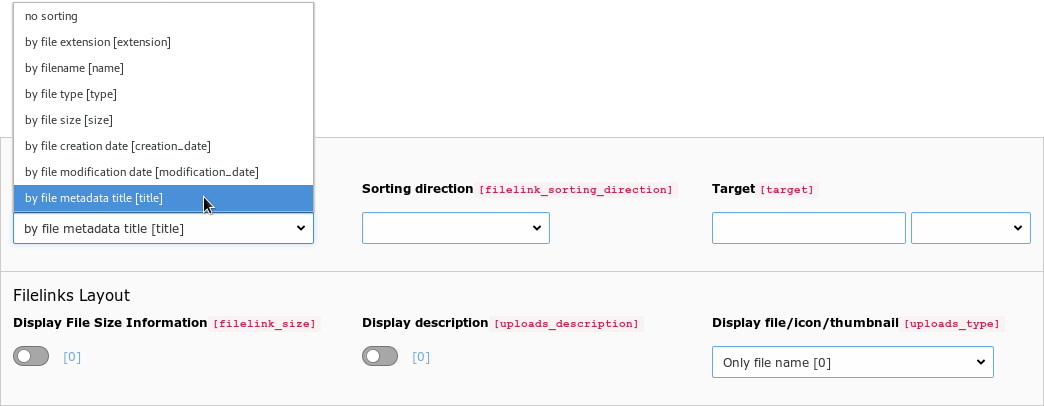
\includegraphics[width=0.90\linewidth]{BackendUserInterface/56213-FilelistSorting.png}
	\end{figure}

\end{frame}

% ------------------------------------------------------------------------------
% Feature | 85569 | Show scheduler information in the system information toolbar

\begin{frame}[fragile]
	\frametitle{Administratorski interfejs}
	\framesubtitle{System Information Toolbar}

	System information toolbar sada prikazuje i informacije vezane za TYPO3 scheduler.

	\begin{figure}
		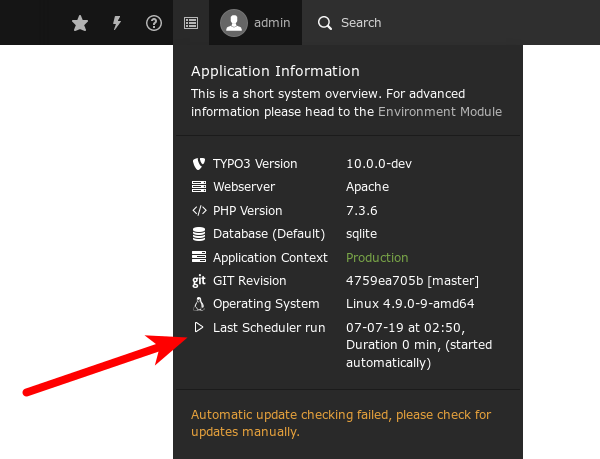
\includegraphics[width=0.50\linewidth]{BackendUserInterface/85569-SchedulerInfoInStatusBar.png}
	\end{figure}

\end{frame}

% ------------------------------------------------------------------------------
% Feature | 86629 | Implement LinkHandler for telephone numbers

\begin{frame}[fragile]
	\frametitle{Administratorski interfejs}
	\framesubtitle{Link Handler}

	Dodat je novi link handler koji omogucava dodavanje linka za telefonske brojeve
	korišcenjem \texttt{tel:} protokola.

	\begin{figure}
		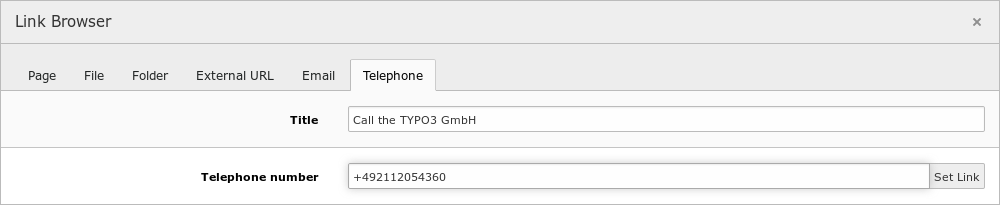
\includegraphics[width=0.90\linewidth]{BackendUserInterface/86629-TelephoneNumberLinkHandler.png}
	\end{figure}

	\begin{figure}
		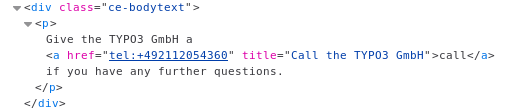
\includegraphics[width=0.60\linewidth]{BackendUserInterface/86629-TelephoneNumberLinkHandler2.png}
	\end{figure}

\end{frame}

% ------------------------------------------------------------------------------
% Feature | 87433 | Add changefreq and priority

\begin{frame}[fragile]
	\frametitle{Administratorski interfejs}
	\framesubtitle{SEO Sitemap (1)}

	\texttt{EXT:seo} sada podržava promenu frekvencije i prioriteta za Sitemap.
	Tab iz osobina strane (tab "SEO") sada ima dva nova polja.

	\begin{figure}
		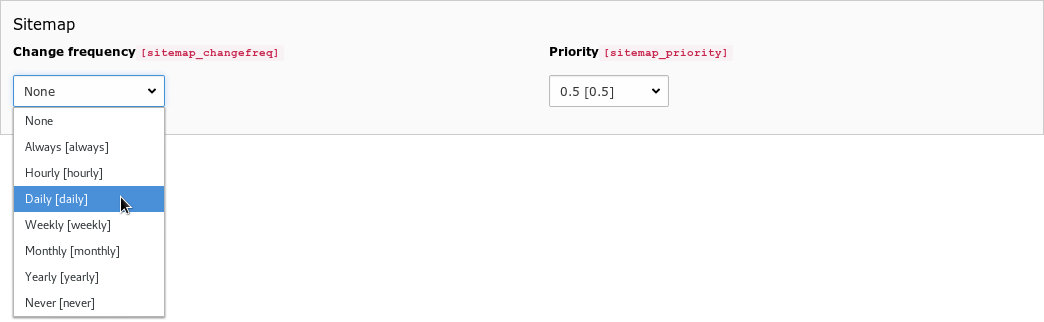
\includegraphics[width=0.90\linewidth]{BackendUserInterface/87433-SeoAddChangefreqAndPriority.png}
	\end{figure}

\end{frame}

% ------------------------------------------------------------------------------
% Feature | 87433 | Add changefreq and priority

\begin{frame}[fragile]
	\frametitle{Administratorski interfejs}
	\framesubtitle{SEO Sitemap (2)}

	% decrease font size for code listing
	\lstset{basicstyle=\tiny\ttfamily}

  Ova podešavanja se mogu, takodje, definisati i u TypoScript-u, mapiranjem na polja
	u bazi podataka.

	\begin{lstlisting}
plugin.tx_seo {
  config {
    xmlSitemap {
      sitemaps {
        <unique key> {
          provider = TYPO3\CMS\Seo\XmlSitemap\RecordsXmlSitemapDataProvider
          config {
            ...
            changeFreqField = news_changefreq
            priorityField = news_priority
            ...
          }
        }
      }
    }
  }
}
	\end{lstlisting}

\end{frame}

% ------------------------------------------------------------------------------
% Feature | 84757 | Double click in structure tree changes label

\begin{frame}[fragile]
	\frametitle{Changes for Integrators}
	\framesubtitle{Forme}

	% decrease font size for code listing
	\lstset{basicstyle=\tiny\ttfamily}

	Labele elemenata se sada mogu menjati duplim klikom na naslov labele u
	pregledu stabla elemenata.

	\begin{figure}
		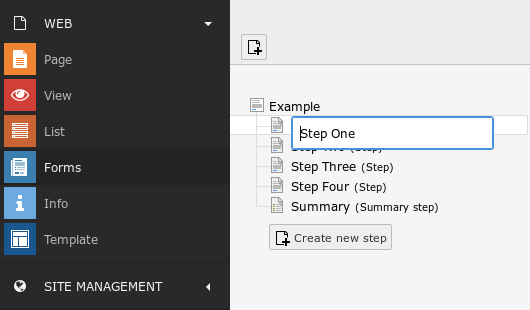
\includegraphics[width=0.60\linewidth]{ChangesForIntegrators/84757-DoubleClickToChangeLabel.png}
	\end{figure}

\end{frame}

% ------------------------------------------------------------------------------
